%% It is just an empty TeX file.
%% Write your code here.
% !TEX encoding = UTF-8 Unicode
\documentclass[a4paper, 12pt]{article}   	% use "amsart" instead of "article" for AMSLaTeX format
\usepackage[left=20mm, top=15mm, right=10mm, bottom=15mm]{geometry}    

            
\usepackage[parfill]{parskip}    		% Activate to begin paragraphs with an empty line rather than an indent
\usepackage{graphicx}				% Use pdf, png, jpg, or eps§ with pdflatex; use eps in DVI mode
\usepackage[14pt]{extsizes}
\usepackage{setspace,amsmath}
\usepackage{ dsfont }
\usepackage{graphicx}
\renewcommand{\labelenumii}{\theenumii}
\renewcommand{\theenumii}{\theenumi.\arabic{enumii}.}
\usepackage{amsmath,amssymb}
\usepackage[unicode]{hyperref}

\usepackage{xcolor}
\usepackage{color}
\usepackage{minted}
\usepackage{caption}

\usepackage{array}
\newcolumntype{P}[1]{>{\centering\arraybackslash}p{#1}}

\usepackage{cmap} % Улучшенный поиск русских слов в полученном pdf-файле
\usepackage[T2A]{fontenc} % Поддержка русских букв
\usepackage[utf8]{inputenc} % Кодировка utf8
\usepackage[english, russian]{babel} % Языки: русский, английский

								% TeX will automatically convert eps --> pdf in pdflatex		
\usepackage{amssymb}

\begin{document}
\begin{titlepage}

\thispagestyle{empty}

\begin{center}
Федеральное государственное бюджетное образовательное учреждение высшего профессионального образования Московский государственный технический университет имени Н.Э. Баумана
\end{center}


\vfill

\centerline{\large{Лабораторная работа №2}}

\centerline{\large{«Триангуляция Делоне»}}

\centerline{\large{по курсу}}
\centerline{\large{«Моделирование»}}


\vfill

Студент группы ИУ9-82 \hfill Белогуров А.А.

Преподаватель \hfill Домрачева А.Б.
\vfill

\centerline{Москва, 2018}
\clearpage
\end{titlepage}

\newpage
\setcounter{page}{2}

\tableofcontents

\newpage

\section{Постановка задачи}
    Изучить различные алгоритмы триангуляции Делоне и реализовать итеративный алгоритм с динамическим кэшированием поиска на произвольном наборе точек.

\newpage

\section{Теоретические сведения}
\subsection{Основные определения}


    \textbf{Триангуляцией} называется планарный граф, все внутренние области которого являются треугольниками. \cite{scvortsov}
    
    \begin{center}
        \begin{minipage}{0.7\linewidth}
            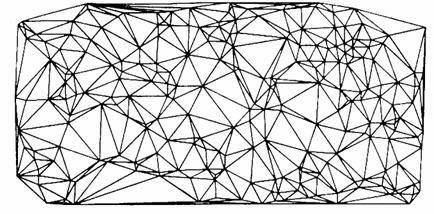
\includegraphics[width=\linewidth]{img/triangulation}
            \captionof{figure}{Пример триангуляции}
        \end{minipage}
    \end{center}
    
    \textbf{Выпуклой триангуляцией} называется такая триангуляция, для которой минимальный многоугольник, охватывающий все треугольники, будет выпуклым. Триангуляция, не являющаяся выпуклой, называется \textbf{невыпуклой}. \cite{scvortsov}
    
    Триангуляция удовлетворяет \textbf{условию Делоне}, если внутрь окружности, описанной вокруг любого построенного треугольника, не попадает ни одна из заданных точек триангуляции. \cite{scvortsov}
    
    Триангуляция называется \textbf{триангуляцией Делоне}, если она является выпуклой и удовлетворяет условию Делоне (Рис. 2)
    
    \begin{center}
        \begin{minipage}{0.5\linewidth}
            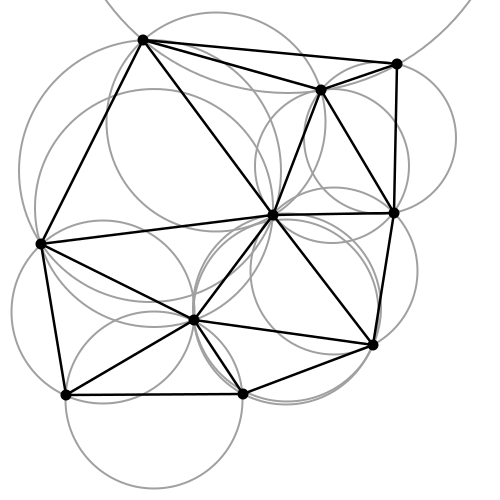
\includegraphics[width=\linewidth]{img/triangulation_delone}
            \captionof{figure}{Триангуляция Делоне}
        \end{minipage}
    \end{center}
    
\subsection{Итеративный алгортим с динамическим кэшированием поиска}

    \begin{enumerate}
        \item Создание суперструктуры, которая будет покрывать все точки. {\it (В данном случае создается прямоугольник, который разбивается диагональю на два треугольника. Следовательно, получаем на этом шаге триангуляцию, которая состоит их двух одинаковых треугольников)}
        \item Выполняем цикл по $n$ точкам для пунктов 3-5.
        \item Очередная $n$-ая точка добавляется в триангуляцию следующим образом. Вначале производится локализация точки с помощью динамического кэша.
        \begin{enumerate}
            \item Если точка попадает в эпсилон-окрестность любой другой вершины триангуляции, то она отбрасывается.
            \item Если точка попала на некоторое ребро, то оно разбивается на два новых, а оба смежных с ребром треугольника также делятся на два меньших. 
            \item Если точка попала строго внутрь какого-нибудь треугольника, он разбивается на три новых.
            \item Если точка попала вне триангуляции, то строится один или более треугольников.  {\it (Так как на первом шаге была построена суперструктура, то все точки заведомо будут лежать внутри нее. Поэтому выполнение этого пункта невозможно)}
        \end{enumerate}
        \item Проводятся локальные проверки вновь полученных треугольников на соответствие условию Делоне и выполняются необходимые перестроения.
    \end{enumerate}
    
    
\newpage

\section{Практическая реализация}
    Далее приведена реализация некоторых методов программы на языке JavaScript, визуализация выполненяется с помощью библиотеки THREE.JS.

\textbf{Листинг 1} Создание суперструктуры.
\begin{minted}[frame=single, framesep=10pt, fontsize = \small, linenos=true, breaklines]{js}
/**
 * Создание суперструктуры, внутри которой будет происходить триангуляция
 * @param {Point} topLeft
 * @param {Point} bottomRight
 */
Triangulation.prototype.createSuperstructure = function(topLeft, bottomRight) {
    // Инициализация двух треугольников
    var left = new Triangle();
    var right = new Triangle();

    var bottomLeft = new Point(topLeft.X, bottomRight.Y);
    var topRight = new Point(bottomRight.X, topLeft.Y);

    // Инициализация ребер суперструктуры
    var diagonal = new Rib(topLeft, bottomRight, left, right);
    var leftRib = new Rib(topLeft, bottomLeft, left, null);
    var rightRib = new Rib(topRight, bottomRight, right, null);
    var topRib = new Rib(topLeft, topRight, right, null);
    var bottomRib = new Rib(bottomLeft, bottomRight, left, null);

    // Определение ребер для треугольников
    left.setRibs(leftRib, bottomRib, diagonal);
    right.setRibs(rightRib, topRib, diagonal);

    // Обновлние струтуры треугольников
    left.update();
    right.update();

    // Добавление треугольников в кэш
    this.cache.initialize(left, right, left, right);

    return [left, right];
};
\end{minted}

\textbf{Листинг 2} Вставка новой точки в триангуляцию
\begin{minted}[frame=single, framesep=10pt, fontsize = \small, linenos=true, breaklines]{js}
/**
 * Вставка новой точки в триангулцию
 * 1) Нахождение треугольника иди ребра, куда попала новая точка
 * 2) Если точка попадает в эпсилон-окрестность любой другой вершины триангуляции - игнорировать ее
 * 3) Если точка попадает на ребро, то треугольники с этим ребром разбиваются на два новых
 * 4) Если точка попадает внутрь треугольника - треугольник разбивается на три новых
 * @param {Point} node Новая точка
 * @returns {array} Массив новых\измененных треугольников
 */
Triangulation.prototype.calcTriangulation = function (node) {
    // Шаг 1)
    var initTriangle = this.cache.get(node);
    var targetTriangle = this.findTriangleBySeparatingRibs(node, initTriangle);

    // Шаг 2)
    for (i = 0; i < targetTriangle.verticies.length; i++) {
        var vert = targetTriangle.verticies[i];
        if (vert.isInEpsilonAreaPoint(node)) {
            return null;
        }
    }

    // Массив новых и измененных треугольников
    var newAndModifiedTriangles = null;
    var newTriangles = null;

    // Шаг 3)
    var targetTriangleRibs = targetTriangle.ribs;
    for (var i = 0; i < targetTriangleRibs.length; i++) {
        if (isInEpsilonArea(distanceToLine(targetTriangleRibs[i].A, targetTriangleRibs[i].B, node), 0)) {
            newAndModifiedTriangles = this.putPointOnRib(targetTriangleRibs[i], node, newTriangles);
            break;
        }
    }

    // Шаг 4)
    if (newAndModifiedTriangles == null) {
        var triangles = this.putPointInTriangle(targetTriangle, node, newTriangles);
        newAndModifiedTriangles = triangles.mdTr;
        newTriangles = triangles.newTr;

    }
    // Увеличение кол-ва вершин в кэше
    this.cache.incrementNodeCount(newTriangles.length);

    // Добавление новых треугольников в кэш
    for (i = 0; i < newTriangles.length; i++) {
        this.cache.update(newTriangles[i]);
    }

    return newAndModifiedTriangles;
};
\end{minted}

\textbf{Листинг 3} Попадание точки внутрь треугольника
\begin{minted}[frame=single, framesep=10pt, fontsize = \small, linenos=true, breaklines]{js}
/**
 * Попадание узла внутрь треугольника
 * @param {Triangle} T
 * @param {Point} node
 * @param {Array<Triangle>} newTriangles
 * @return {Array<Triangle>} Измененные треугольники
 */
Triangulation.prototype.putPointInTriangle = function(T, node, newTriangles){
    // Вершины
    // node == O
    var A = T.verticies[0];
    var B = T.verticies[1];
    var C = T.verticies[2];

    // Треугольники
    var LT = new Triangle();
    var RT = new Triangle();

    newTriangles = [LT, RT];

    // Ребра
    var AB = T.getRib(A, B);
    var BC = T.getRib(B, C);
    var AC = T.getRib(A, C);

    // Новые ребра.
    var OA = new Rib(node, A, LT, T);
    var OB = new Rib(node, B, LT, RT);
    var OC = new Rib(node, C, RT, T);

    // Обновление ссылок на смежные треугольники
    AB.update(T, LT);
    BC.update(T, RT);

    // Обновление старых ребер на новые
    T.updateRib(AB, OA);
    T.updateRib(BC, OC);

    // Определение новых ребер треугольника
    LT.setRibs(AB, OB, OA);
    RT.setRibs(BC, OB, OC);

    // Добавление новых треугольников в триангуляцию
    this.triangles.push(LT);
    this.triangles.push(RT);

    // Обновление структур треугольников
    T.update();
    LT.update();
    RT.update();

    var modifiedTriangles = [T, LT, RT];
    // Return new and modified triangles.
    return {
        newTr: newTriangles,
        mdTr: modifiedTriangles
    }
};
\end{minted}

\textbf{Листинг 4} Локализация точки
\begin{minted}[frame=single, framesep=10pt, fontsize = \small, linenos=true, breaklines]{js}
/**
 * Найти треугольник в кэше по точке
 * @param {Point} node Точка
 * @return {Triangle} Треугольник из кэша
 */
DynamicCache.prototype.get = function(node)
{
    var row = this.getRow(node.Y);
    var col = this.getCol(node.X);
    return this.cache[row][col];
};
\end{minted}

\newpage
\section{Результаты}
    Далее будут приведены результаты программы на разном количестве данных. 
    
    \textbf{С отображением суперструктуры:}
    \begin{center}
        \begin{minipage}{0.47\linewidth}
            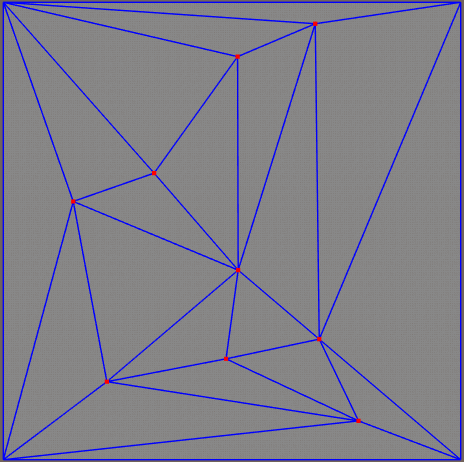
\includegraphics[width=\linewidth]{img/triang_super_9}
            \captionof{figure}{9 точек}
        \end{minipage}
        \begin{minipage}{0.47\linewidth}
            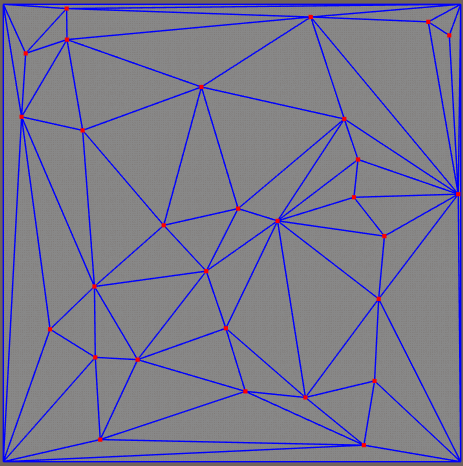
\includegraphics[width=\linewidth]{img/triang_super_29}
            \captionof{figure}{29 точек}
        \end{minipage}
        \begin{minipage}{0.47\linewidth}
            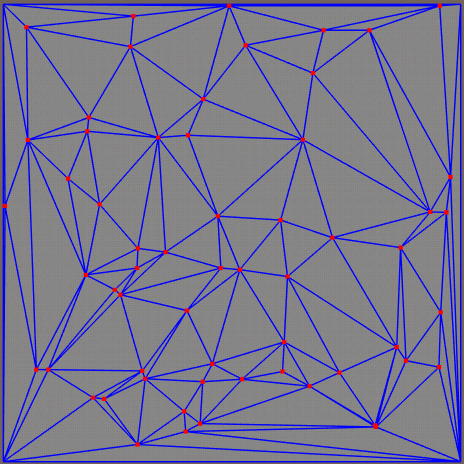
\includegraphics[width=\linewidth]{img/triang_super_59}
            \captionof{figure}{59 точек}
        \end{minipage}
    \end{center}
    
    \textbf{Без отображениея суперструктуры:}
    \begin{center}
        \begin{minipage}{0.47\linewidth}
            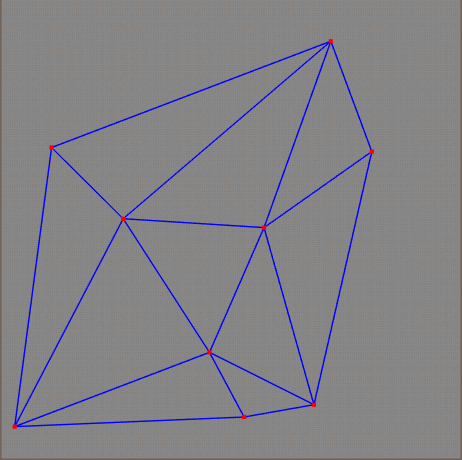
\includegraphics[width=\linewidth]{img/triang_9}
            \captionof{figure}{9 точек}
        \end{minipage}
        \begin{minipage}{0.47\linewidth}
            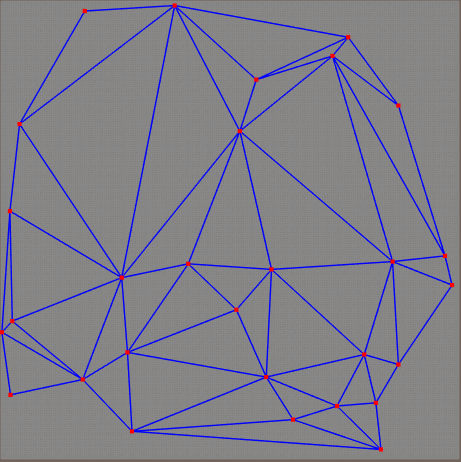
\includegraphics[width=\linewidth]{img/triang_29}
            \captionof{figure}{29 точек}
        \end{minipage}
        \begin{minipage}{0.47\linewidth}
            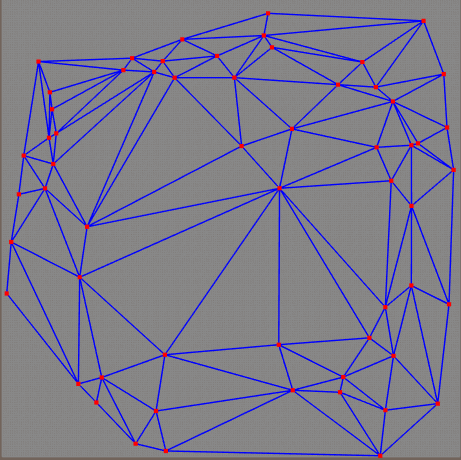
\includegraphics[width=\linewidth]{img/triang_59}
            \captionof{figure}{59 точек}
        \end{minipage}
    \end{center}

\newpage
\section{Вывод}
    В ходе выполнения лабораторной работы было изучены алгоритмы построения триангуляции Делоне и реализован итеративный алгоритм с динамическим кэшированием поиска. Он выигрывает по быстродействию у всех существующих, так как имеют динамическую структуру - кэш, который служит для быстрой локализации точки. Данный факт был подтвержден для большого количества данных.

\newpage

\bibliographystyle{utf8gost705u}  %% стилевой файл для оформления по ГОСТу
\bibliography{biblio} 
\addcontentsline{toc}{section}{Список используемой литературы}

\end{document} 














